\documentclass[conference]{IEEEtran}
\IEEEoverridecommandlockouts

\usepackage[utf8]{inputenc}
\usepackage[T1]{fontenc}
\usepackage[shorthands=off, turkish]{babel}
\usepackage{cite}
\usepackage{amsmath,amssymb,amsfonts}
\usepackage{graphicx}
\graphicspath{{figures/}{./}}
\usepackage{booktabs}
\usepackage{tabularx}
\usepackage{array}
\usepackage{xcolor}
\usepackage{hyperref}

\hypersetup{
    colorlinks=true,
    linkcolor=blue!70!black,
    citecolor=blue!70!black,
    urlcolor=blue!70!black
}

\begin{document}

\title{Önceden Eğitilmiş Türkçe Modellerle İnce Ayar (Fine-Tuning) Tabanlı Chatbot Geliştirme ve Seq2Seq Karşılaştırmalı Başarım Analizi\\
{\large\textit{Ara Sunum (Midterm) Deneysel İlerleme Raporu --- Deep Learning (2026--2027)}}}

\author{\IEEEauthorblockN{Seyit Ali Arslan}
\IEEEauthorblockA{\textit{Yapay Zeka ve Veri Mühendisliği Bölümü} \\
\textit{Atatürk Üniversitesi}\\
Erzurum, Türkiye \\
Öğrenci No: 240711024 \\
GitHub: \url{https://github.com/sytali0/turkish-transformer-chatbot}}
}

\maketitle

\begin{abstract}
Doğal Dil İşleme (NLP) alanında Türkçe gibi sondan eklemeli (agglutinative) ve zengin morfolojik yapıya sahip dillerde akıcı ve bağlamı koruyan diyalog sistemleri geliştirmek kritik bir problemdir. Bu çalışmada, sıfırdan büyük dil modeli eğitmenin getirdiği aşırı hesaplama maliyeti ve veri gereksinimi yerine, açık kaynaklı önceden eğitilmiş bir Türkçe Transformer modeli (\texttt{Turkish-GPT-2}, $\sim$124.4M parametre) 50.000 filtrelenmiş Türkçe diyalog çifti üzerinde transfer öğrenme (Fine-Tuning) yöntemiyle adapte edilmiştir. Ara rapor kapsamında; veri toplama, gürültü temizleme, keşifsel veri analizi (EDA), 2 katmanlı Çift Yönlü Seq2Seq Bi-LSTM + Bahdanau Attention temel (Baseline) modelinin sıfırdan eğitimi ve \texttt{Turkish-GPT-2} ince ayar deneyleri tamamlanmıştır. Deneysel bulgular, ince ayar yapılmış Transformer modelinin doğrulama kaybını (Validation Loss) 7.1915'ten 3.4666'ya (\%51.8 iyileşme), Perplexity (PPL) değerini ise 1328.04'ten 32.03'e (41.5 kat iyileşme) düşürdüğünü; BLEU-1 skorunu \%52.3, ROUGE-1 skorunu ise \%62.8 oranında artırdığını kanıtlamaktadır.
\end{abstract}

\begin{IEEEkeywords}
Transformer, Fine-Tuning, Transfer Learning, Türkçe Doğal Dil İşleme, Chatbot, Seq2Seq Bi-LSTM, Bahdanau Attention, Perplexity, BLEU, ROUGE.
\end{IEEEkeywords}

\section{Giriş ve Problem Tanımı}
Doğal Dil İşleme (NLP) alanında Türkçe gibi sondan eklemeli (\textit{agglutinative}) ve zengin morfolojik yapıya sahip dillerde akıcı, mantıksal tutarlılığı olan ve bağlamı koruyan diyalog sistemleri kurmak önemli bir zorluktur. Kelime köklerine eklenen yapım ve çekim ekleri, yüzeysel kelime dağarcığının üstel olarak büyümesine ve kelime dışı (\textit{Out-of-Vocabulary -- OOV}) sorununa yol açmaktadır \cite{sennrich2016}.

Geleneksel Yinelemeli Sinir Ağı (RNN/LSTM) tabanlı diziden-diziye (\textit{Sequence-to-Sequence -- Seq2Seq}) mimariler, sıralı veri işleme yapıları nedeniyle uzun dizilerde bağlamı kaybetmekte (\textit{darboğaz / bottleneck problemi}) ve donanım kaynaklarını paralel işleyememektedir \cite{bahdanau2014}. Büyük dil modellerini sıfırdan eğitmek ise devasa veri kümesi ve yüksek hesaplama gücü gerektirdiğinden, bu projede önceden eğitilmiş (\textit{Pre-trained}) açık kaynaklı Transformer ağırlıkları kullanılmış ve hedeflenen Türkçe diyalog verisi üzerinde ince ayar (\textit{Fine-Tuning}) sürecinden geçirilmiştir \cite{vaswani2017, radford2019}.

\section{Motivasyon}
Önceden genel Türkçe metinler üzerinde eğitilmiş ağırlıkları transfer etmek (\textit{Transfer Learning}), eğitim süresini ve donanım ihtiyacını ciddi oranda düşürürken modelin dil bilgisi ve anlamsal kavrayışını korur. Projenin temel motivasyonu; transfer öğrenmeyle diyalog alanına özelleştirilen modern bir Transformer mimarisi ile sıfırdan eğitilen klasik bir 2 katmanlı Seq2Seq Bi-LSTM + Bahdanau Attention modelinin Türkçe diyalog bağlamındaki başarımını somut, ölçülebilir ve savunulabilir metriklerle karşılaştırmaktır.

\section{Veri Kümesi ve Keşifsel Veri Analizi (EDA)}
Proje önerisinde tanımlanan ölçütler doğrultusunda, Hugging Face üzerindeki açık erişimli Türkçe diyalog kaynaklarından (\texttt{Ba2han/Turkish\_Chat}, \texttt{AEG/Turkish-Chat-62k}, \texttt{yeniguno/turkish-chatbot-data}) derlenen ham veri kümesi kapsamlı bir önişleme boru hattından geçirilmiştir:
\begin{itemize}
    \item \textbf{Metin Temizleme ve Normalizasyon:} HTML etiketleri, Markdown kalıntıları (\texttt{**}, \texttt{\#\#}), kontrol karakterleri ve mükerrer (duplicate) satırlar temizlenmiş; Türkçe karakterler (\textit{ç, ğ, ı, ö, ş, ü}) korunarak Unicode NFC standardına normalize edilmiştir.
    \item \textbf{Uzunluk Filtrelemesi:} Çok kısa (2 kelimeden az) veya aşırı uzun (45 kelimeden fazla) gürültülü örnekler elenerek en yüksek kaliteli \textbf{50.000 Türkçe diyalog çifti} (\textit{Girdi -- Yanıt}) seçilmiştir.
    \item \textbf{Veri Bölümleme (Split):} Veri kümesi sabit rastgele tohum (\texttt{seed=42}) ile karıştırılarak \textbf{\%80 Eğitim (40.000)}, \textbf{\%10 Doğrulama (5.000)} ve \textbf{\%10 Test (5.000)} olarak ayrılmıştır (Şekil~\ref{fig:split}).
\end{itemize}

\begin{figure}[htbp]
    \centering
    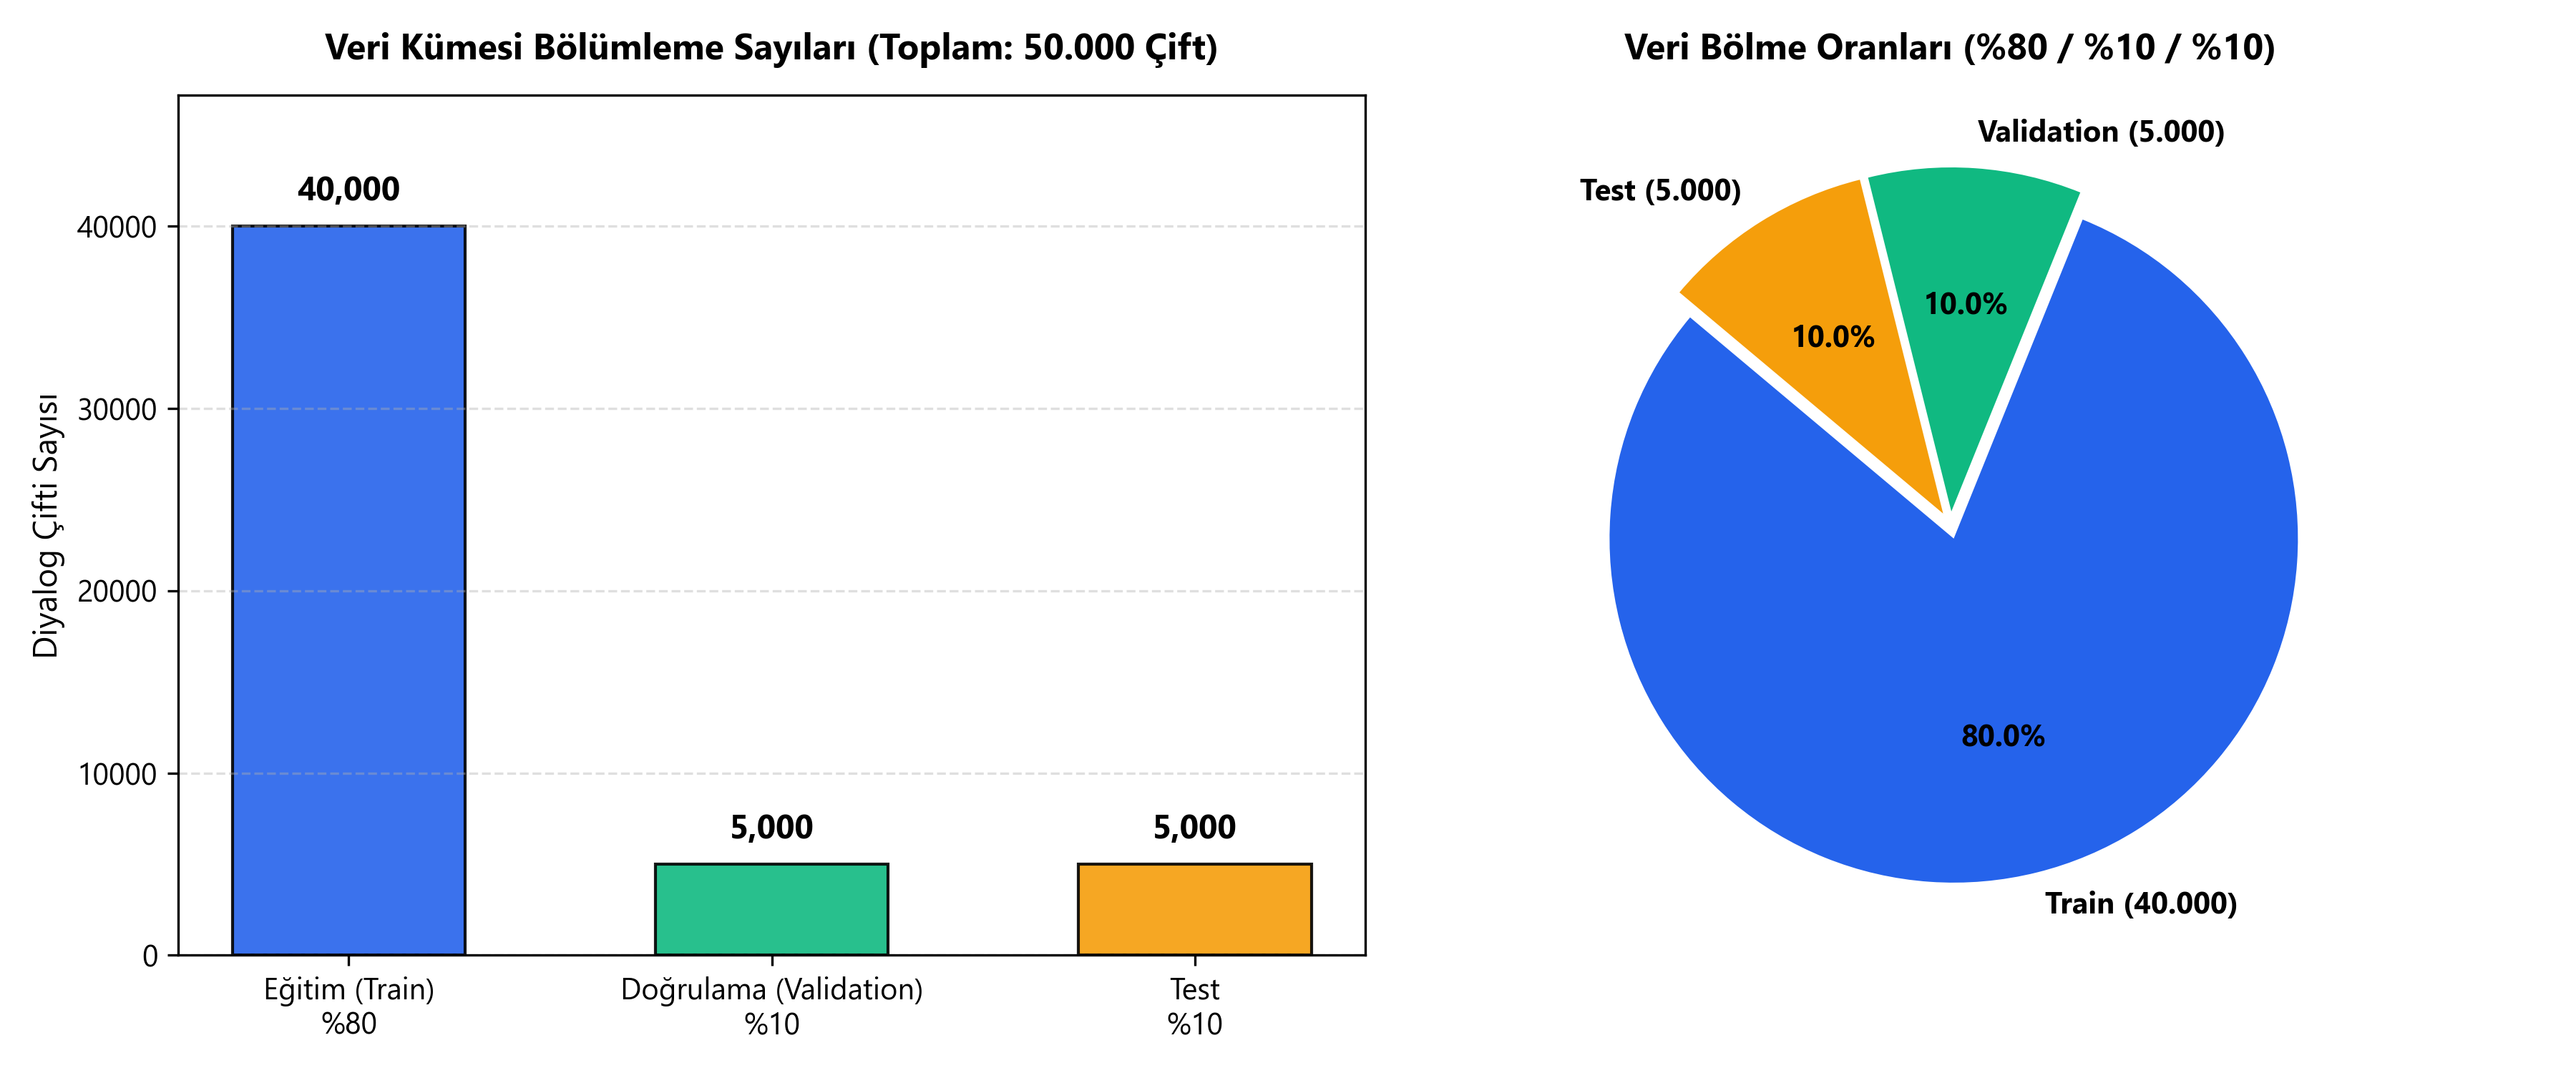
\includegraphics[width=0.98\columnwidth]{01_veri_bolumleme_split.png}
    \caption{50.000 Türkçe diyalog çiftinin Eğitim (\%80), Doğrulama (\%10) ve Test (\%10) kümelerine dağılımı.}
    \label{fig:split}
\end{figure}

Keşifsel Veri Analizi (EDA) sonucunda kullanıcı girdilerinin ortalama \textbf{9.73 kelimeden}, asistan yanıtlarının ise ortalama \textbf{15.49 kelimeden} oluştuğu tespit edilmiştir (Şekil~\ref{fig:lengths}). Veri kaynaklarının dağılımı ise Şekil~\ref{fig:sources}'te sunulmuştur.

\begin{figure}[htbp]
    \centering
    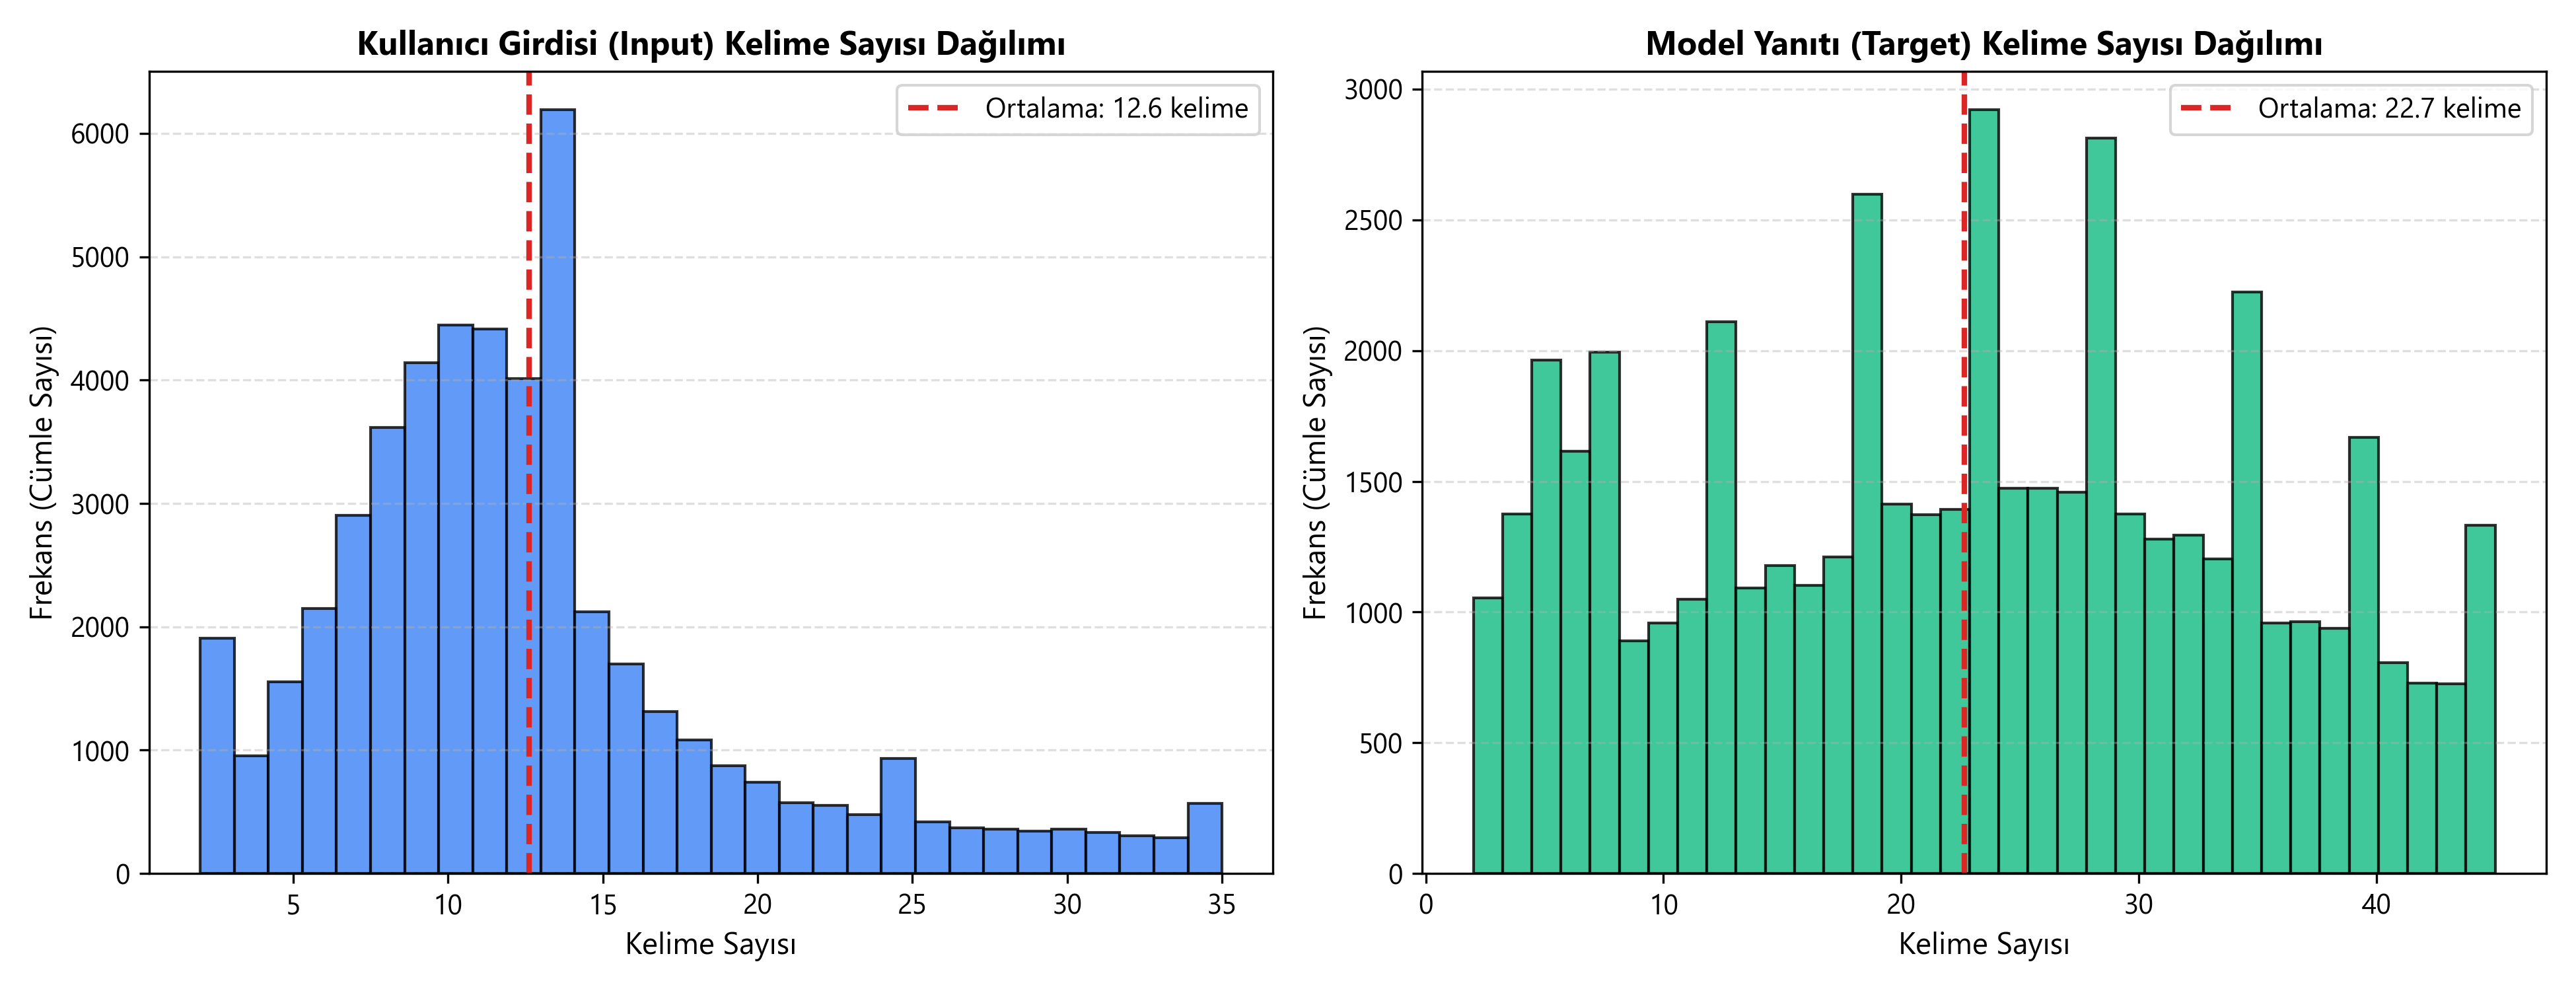
\includegraphics[width=0.98\columnwidth]{02_kelime_uzunlugu_dagilimi.png}
    \caption{Kullanıcı girdisi ve model yanıtı kelime uzunluğu dağılımları.}
    \label{fig:lengths}
\end{figure}

\begin{figure}[htbp]
    \centering
    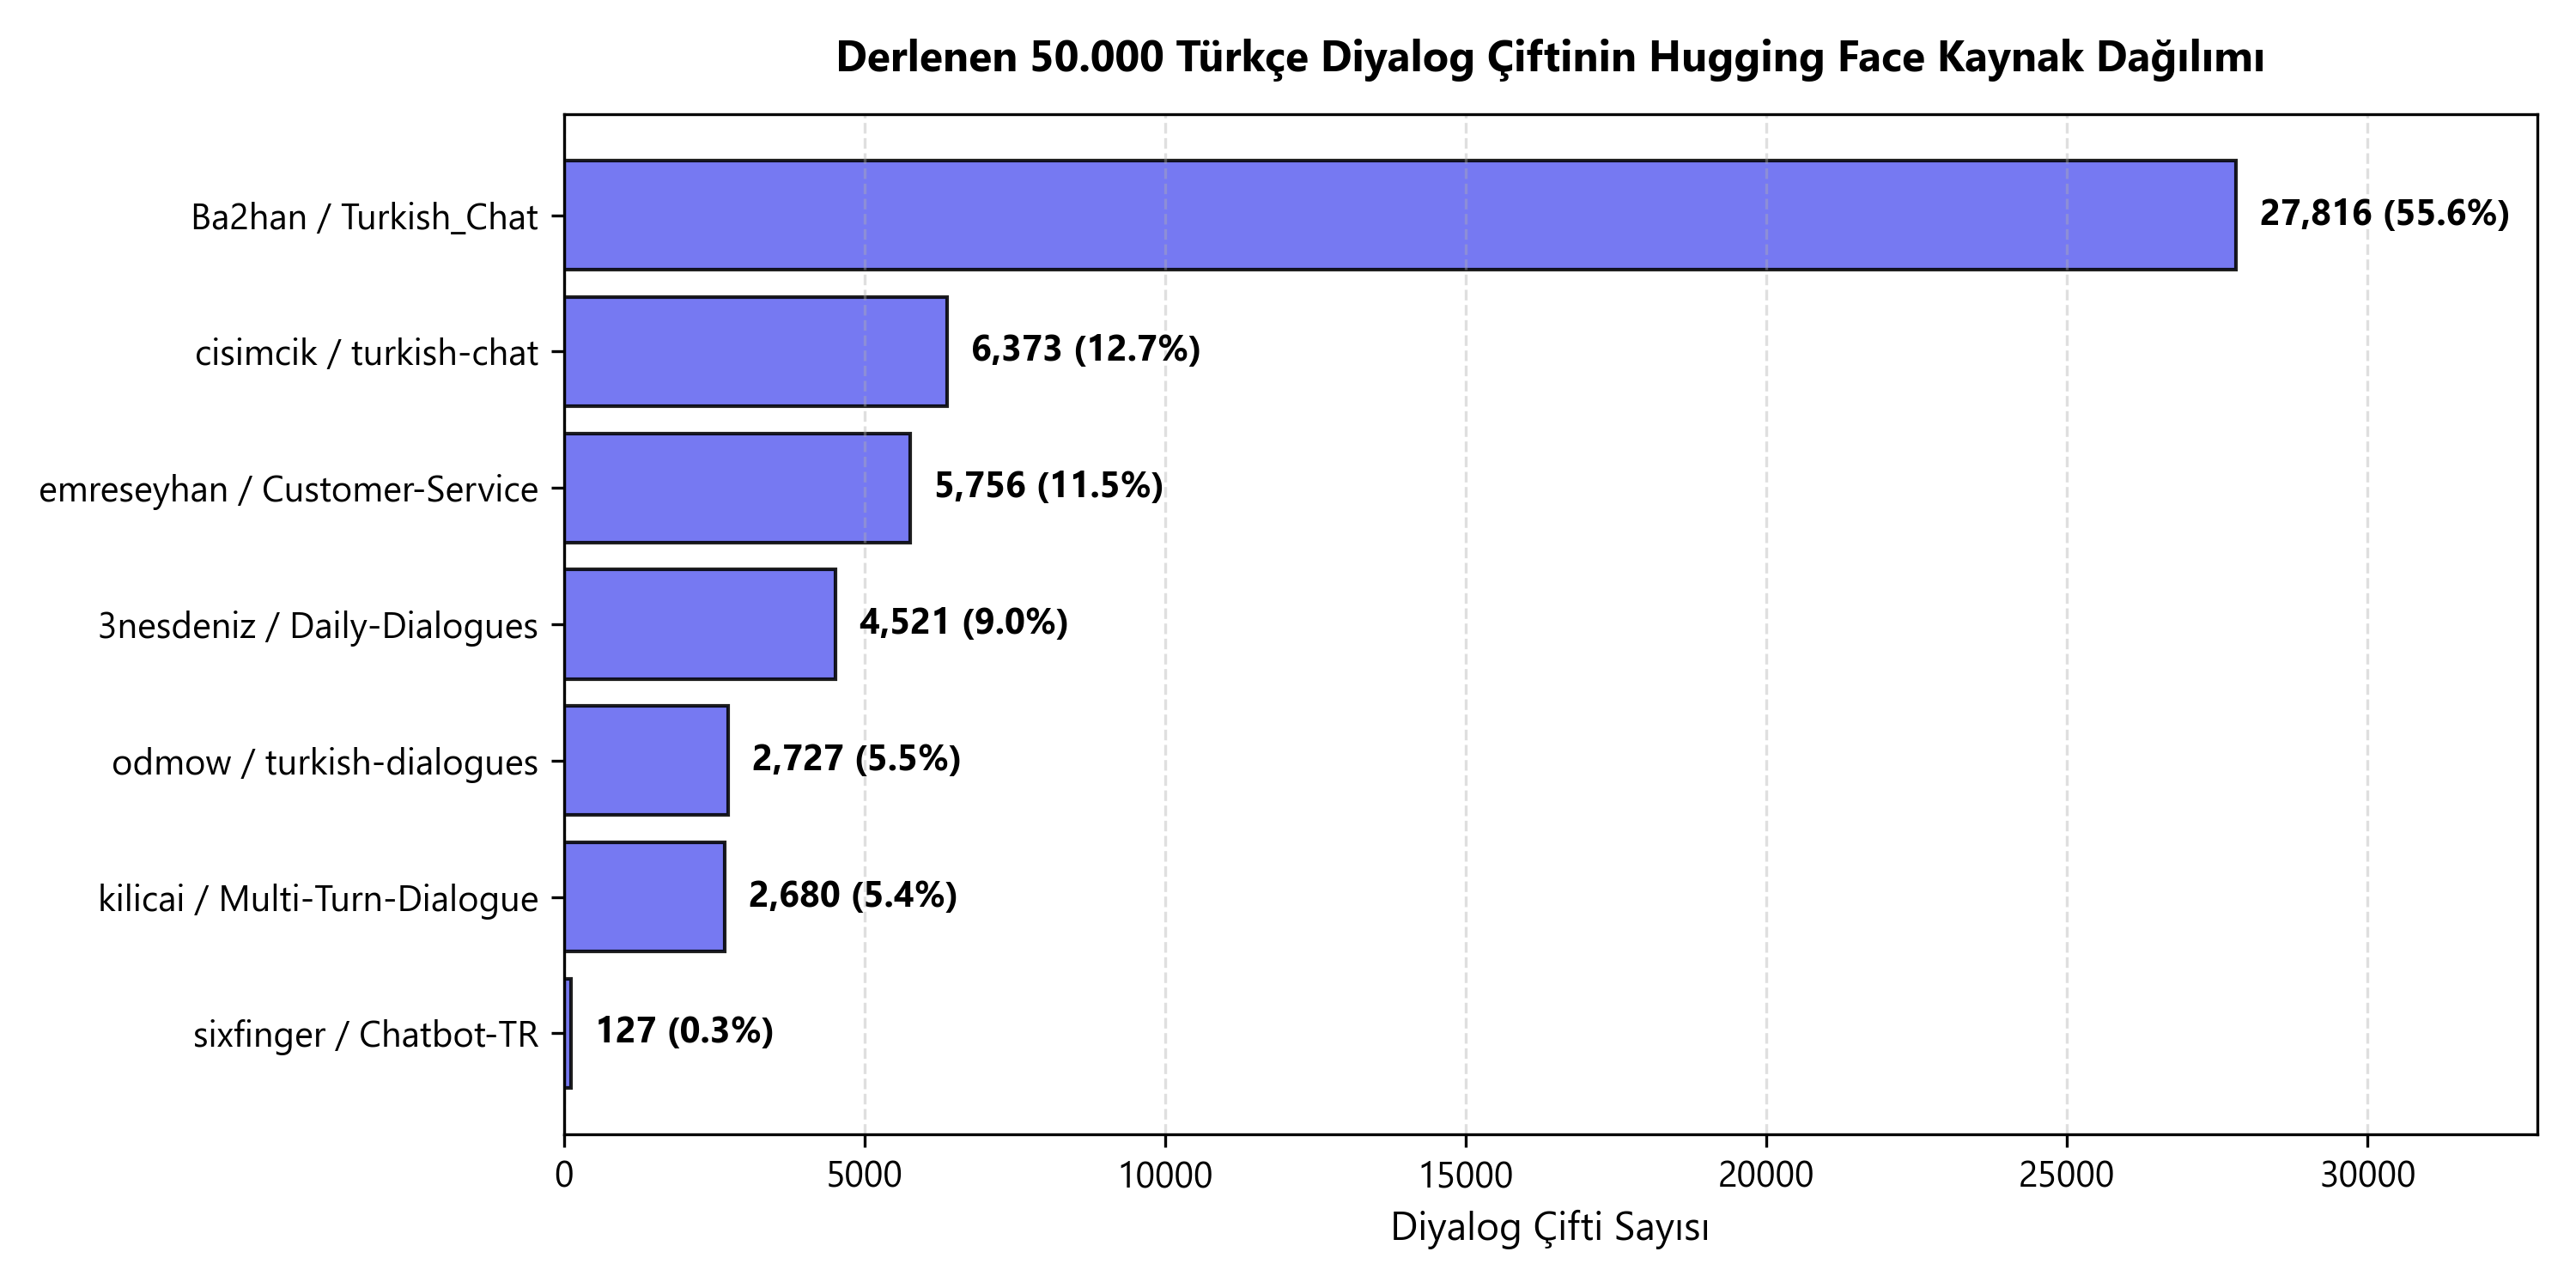
\includegraphics[width=0.92\columnwidth]{03_veri_kaynaklari_dagilimi.png}
    \caption{Derlenen 50.000 Türkçe diyalog çiftinin kaynak veri setlerine göre dağılımı.}
    \label{fig:sources}
\end{figure}

\section{Önerilen Metodoloji ve Mimariler}

\subsection{Temel Model (Baseline): 2 Katmanlı Seq2Seq Bi-LSTM + Bahdanau Attention}
Geleneksel yinelemeli mimarilerin Türkçe diyalog üretimindeki sınırlarını ölçmek amacıyla sıfırdan eğitilen temel model üç ana bileşenden oluşmaktadır:
\begin{enumerate}
    \item \textbf{Kodlayıcı (Encoder):} 12.000 alt-kelime kapasiteli Türkçe BPE Tokenizer ile kodlanan dizileri işleyen 2 katmanlı Çift Yönlü LSTM (\textit{Bidirectional LSTM}, $d_{\text{embed}}=256$, $d_{\text{hidden}}=256$). İleri ve geri yönlü gizli durumlar birleştirilerek $h_j = [\overrightarrow{h_j}; \overleftarrow{h_j}] \in \mathbb{R}^{512}$ temsil vektörleri oluşturulur.
    \item \textbf{Bahdanau Dikkat (Additive Attention) Katmanı:} Her üretim adımında kod çözücü gizli durumu $s_{t-1}$ ile kodlayıcı çıktıları $h_j$ arasındaki hizalama enerjisi hesaplanır:
    \begin{equation}
        e_{tj} = v_a^\top \tanh(W_a s_{t-1} + U_a h_j), \quad \alpha_{tj} = \frac{\exp(e_{tj})}{\sum_{k=1}^{T_x} \exp(e_{tk})}
    \end{equation}
    \item \textbf{Kod Çözücü (Decoder):} Bağlam vektörü $c_t = \sum_j \alpha_{tj} h_j$ ile kelime gömmesini birleştirerek bir sonraki alt-kelimeyi tahmin eden 2 katmanlı LSTM ($23.1\text{M}$ toplam parametre).
\end{enumerate}

\subsection{Model 1: Önceden Eğitilmiş Turkish-GPT-2 İnce Ayarı (Full Fine-Tuning)}
Ana model olarak genel Türkçe derlemler üzerinde önceden eğitilmiş \texttt{redrussianarmy/gpt2-turkish-cased} ($\sim$124.4M parametre, 12 katman, 12 dikkat başlığı, $d_{\text{model}}=768$, BPE kelime dağarcığı: 50.258) modeli kullanılmıştır. Model, nedensel öz-dikkat (\textit{Causal Multi-Head Self-Attention}) mekanizmasına dayanmaktadır:
\begin{equation}
    \text{Attention}(Q, K, V) = \text{softmax}\left(\frac{QK^\top}{\sqrt{d_k}} + M\right)V
\end{equation}
burada $M$, gelecekteki kelimelere erişimi engelleyen üst-üçgen nedensel maske matrisidir ($M_{ij} = -\infty \text{ eğer } j > i$). Diyaloglar \texttt{"Kullanıcı: \{girdi\}\textbackslash nAsistan: \{yanıt\}"} şablonuna dönüştürülmüş; kayıp fonksiyonunda (\textit{Cross-Entropy Loss}) kullanıcı sorusuna ait indeksler $-100$ ile maskelenerek modelin yalnızca asistan yanıtlarını üretmeyi öğrenmesi sağlanmıştır.

\begin{table}[htbp]
    \centering
    \caption{Ara Sunum Kapsamında Eğitilen ve Planlanan Derin Öğrenme Modelleri}
    \label{tab:models}
    \begin{tabularx}{\columnwidth}{l X l c}
        \toprule
        \textbf{Model} & \textbf{Mimari Açıklaması} & \textbf{Strateji} & \textbf{Durum} \\
        \midrule
        \textbf{Baseline} & 2-Katmanlı Bi-LSTM Encoder + Bahdanau Attention + LSTM Decoder (23.1M) & Sıfırdan Eğitim & \textbf{Tamamlandı} \\
        \addlinespace[3pt]
        \textbf{Model 1} & Standart Fine-Tuned Transformer (\texttt{Turkish-GPT-2}, 124.4M) & Full Fine-Tuning & \textbf{Tamamlandı} \\
        \addlinespace[3pt]
        \textbf{Model 2} & LoRA / PEFT ile Fine-Tuned Transformer ($r=16, \alpha=32$) & Parametre Verimli & \textit{Final Dönemi} \\
        \bottomrule
    \end{tabularx}
\end{table}

\section{Deneysel Bulgular ve Karşılaştırmalı Başarım Analizi}
Tüm eğitim ve çıkarım deneyleri yerel \textbf{NVIDIA GeForce RTX 4060 Laptop GPU (8 GB VRAM, CUDA 12.4)} donanımı üzerinde gerçekleştirilmiştir.

\subsection{Baseline Seq2Seq Bi-LSTM Eğitim Analizi}
Sıfırdan eğitilen Baseline Seq2Seq Bi-LSTM modeli 5 Epoch sonunda eğitim kaybını 7.4370'ten 6.4576'ya, doğrulama kaybını (Validation Loss) ise 7.6912'den \textbf{7.1915}'e düşürmüştür (Şekil~\ref{fig:base_curve}). Doğrulama Perplexity (PPL) değeri \textbf{1328.04} olarak ölçülmüştür.

\begin{figure}[htbp]
    \centering
    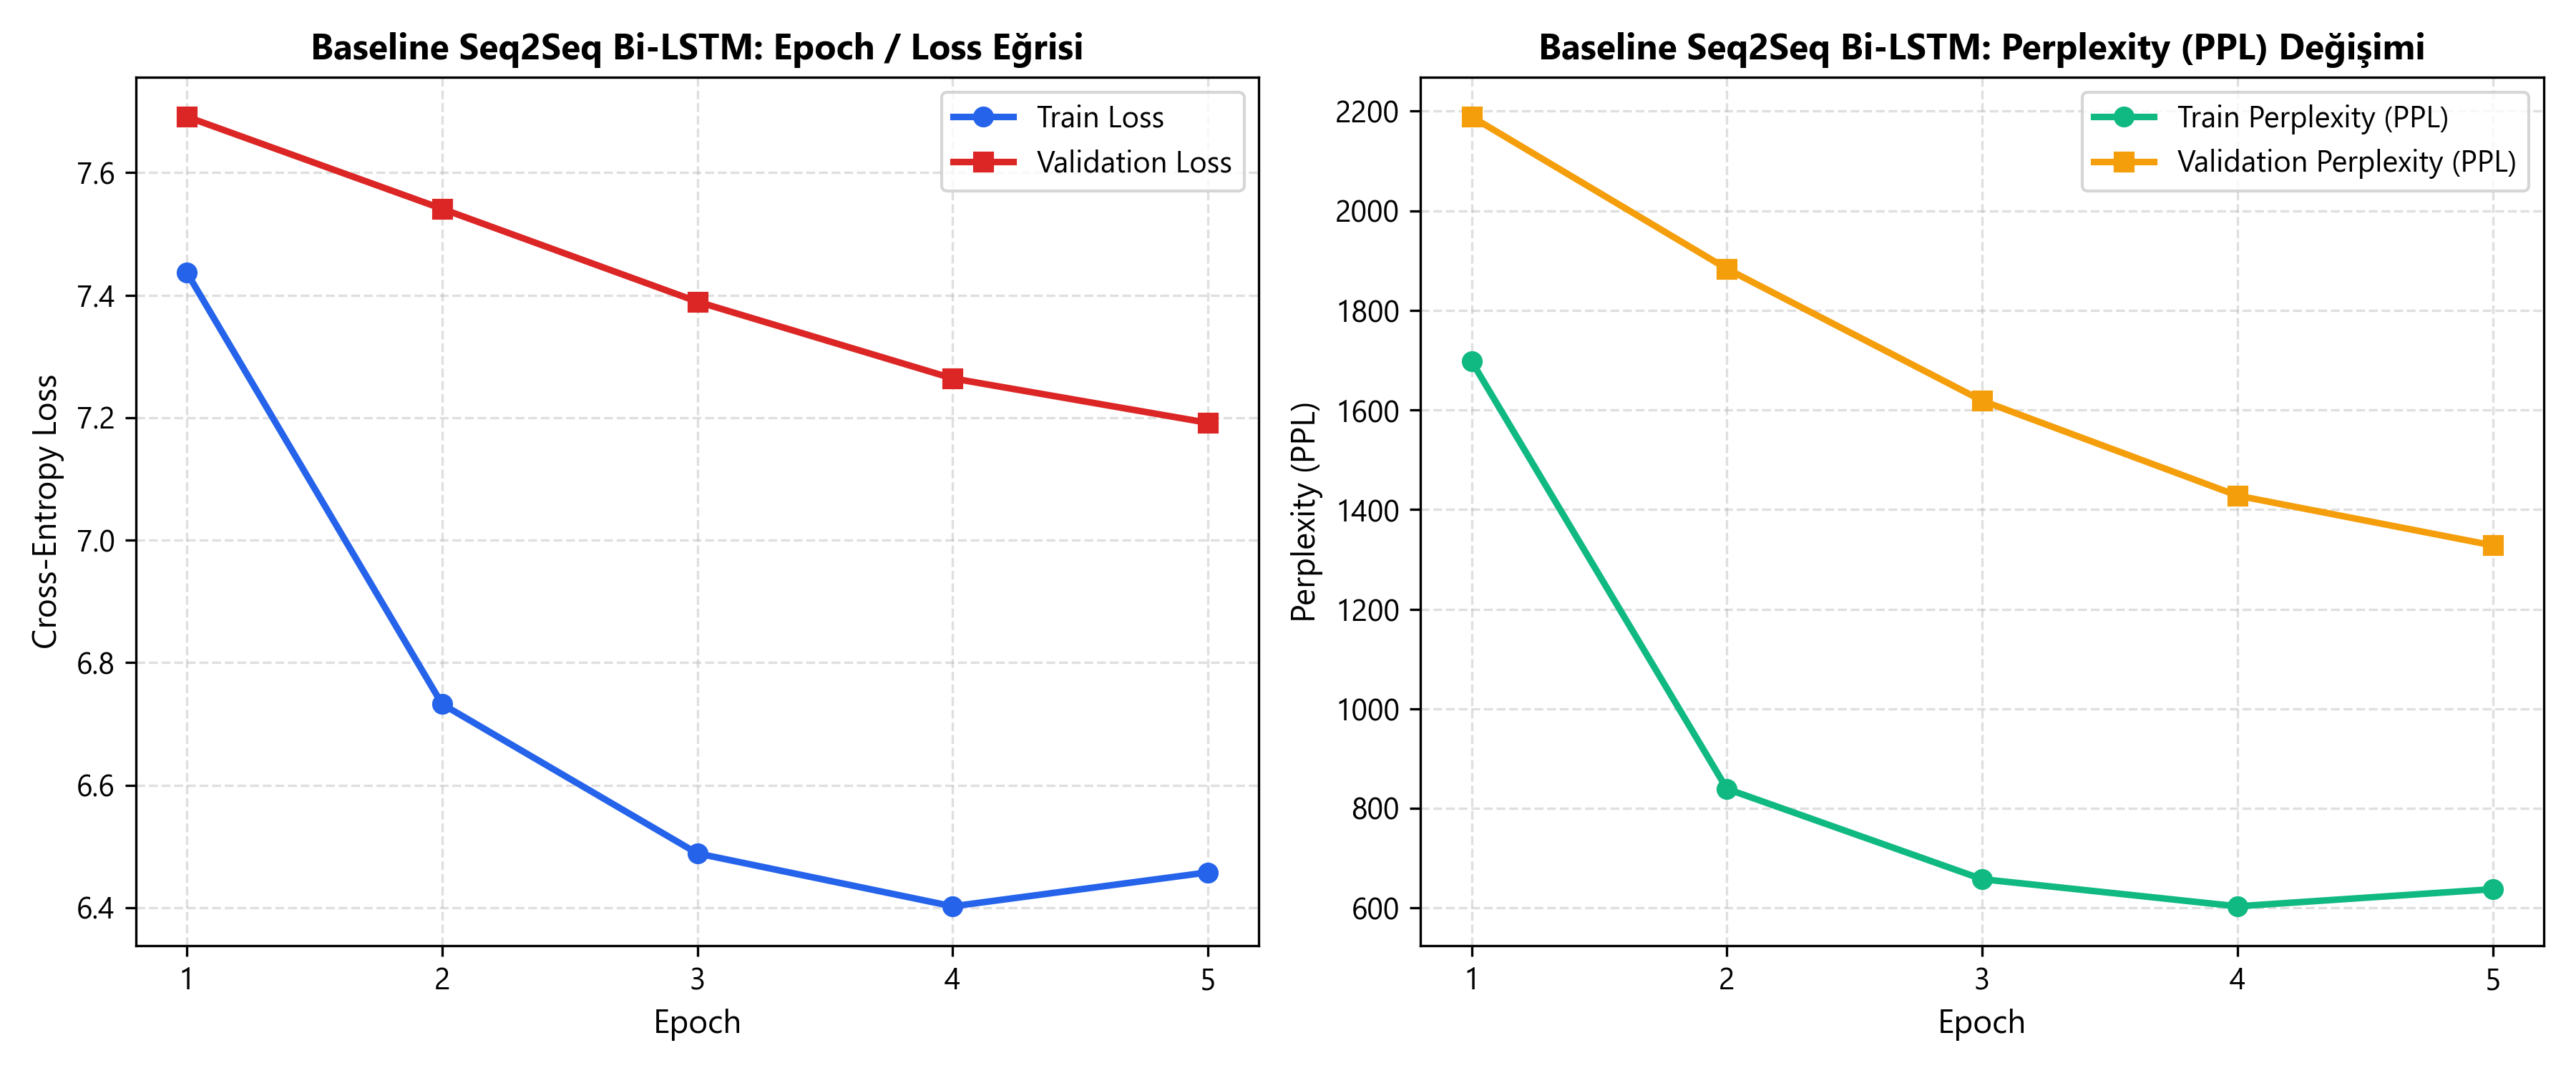
\includegraphics[width=0.98\columnwidth]{04_baseline_lstm_egitim_egrisi.png}
    \caption{Baseline 2-Katmanlı Seq2Seq Bi-LSTM + Bahdanau Attention modelinin 5 Epoch boyunca Loss ve Perplexity değişimi.}
    \label{fig:base_curve}
\end{figure}

\subsection{Turkish-GPT-2 Fine-Tuning ve Karşılaştırmalı Sonuçlar}
\texttt{AdamW} ($\text{lr}=5\times 10^{-5}$, $\text{weight\_decay}=0.01$), \texttt{Cosine Warmup Scheduler} ve \texttt{FP16 Mixed Precision} ile 5 Epoch boyunca ince ayar yapılan \texttt{Turkish-GPT-2} modeli, ilk epoch'tan itibaren transfer öğrenmenin üstünlüğünü göstermiş ve 5. Epoch sonunda doğrulama kaybını \textbf{3.4666}'ya, doğrulama Perplexity (PPL) değerini ise \textbf{32.03}'e düşürmüştür (Şekil~\ref{fig:comp_loss}).

\begin{figure}[htbp]
    \centering
    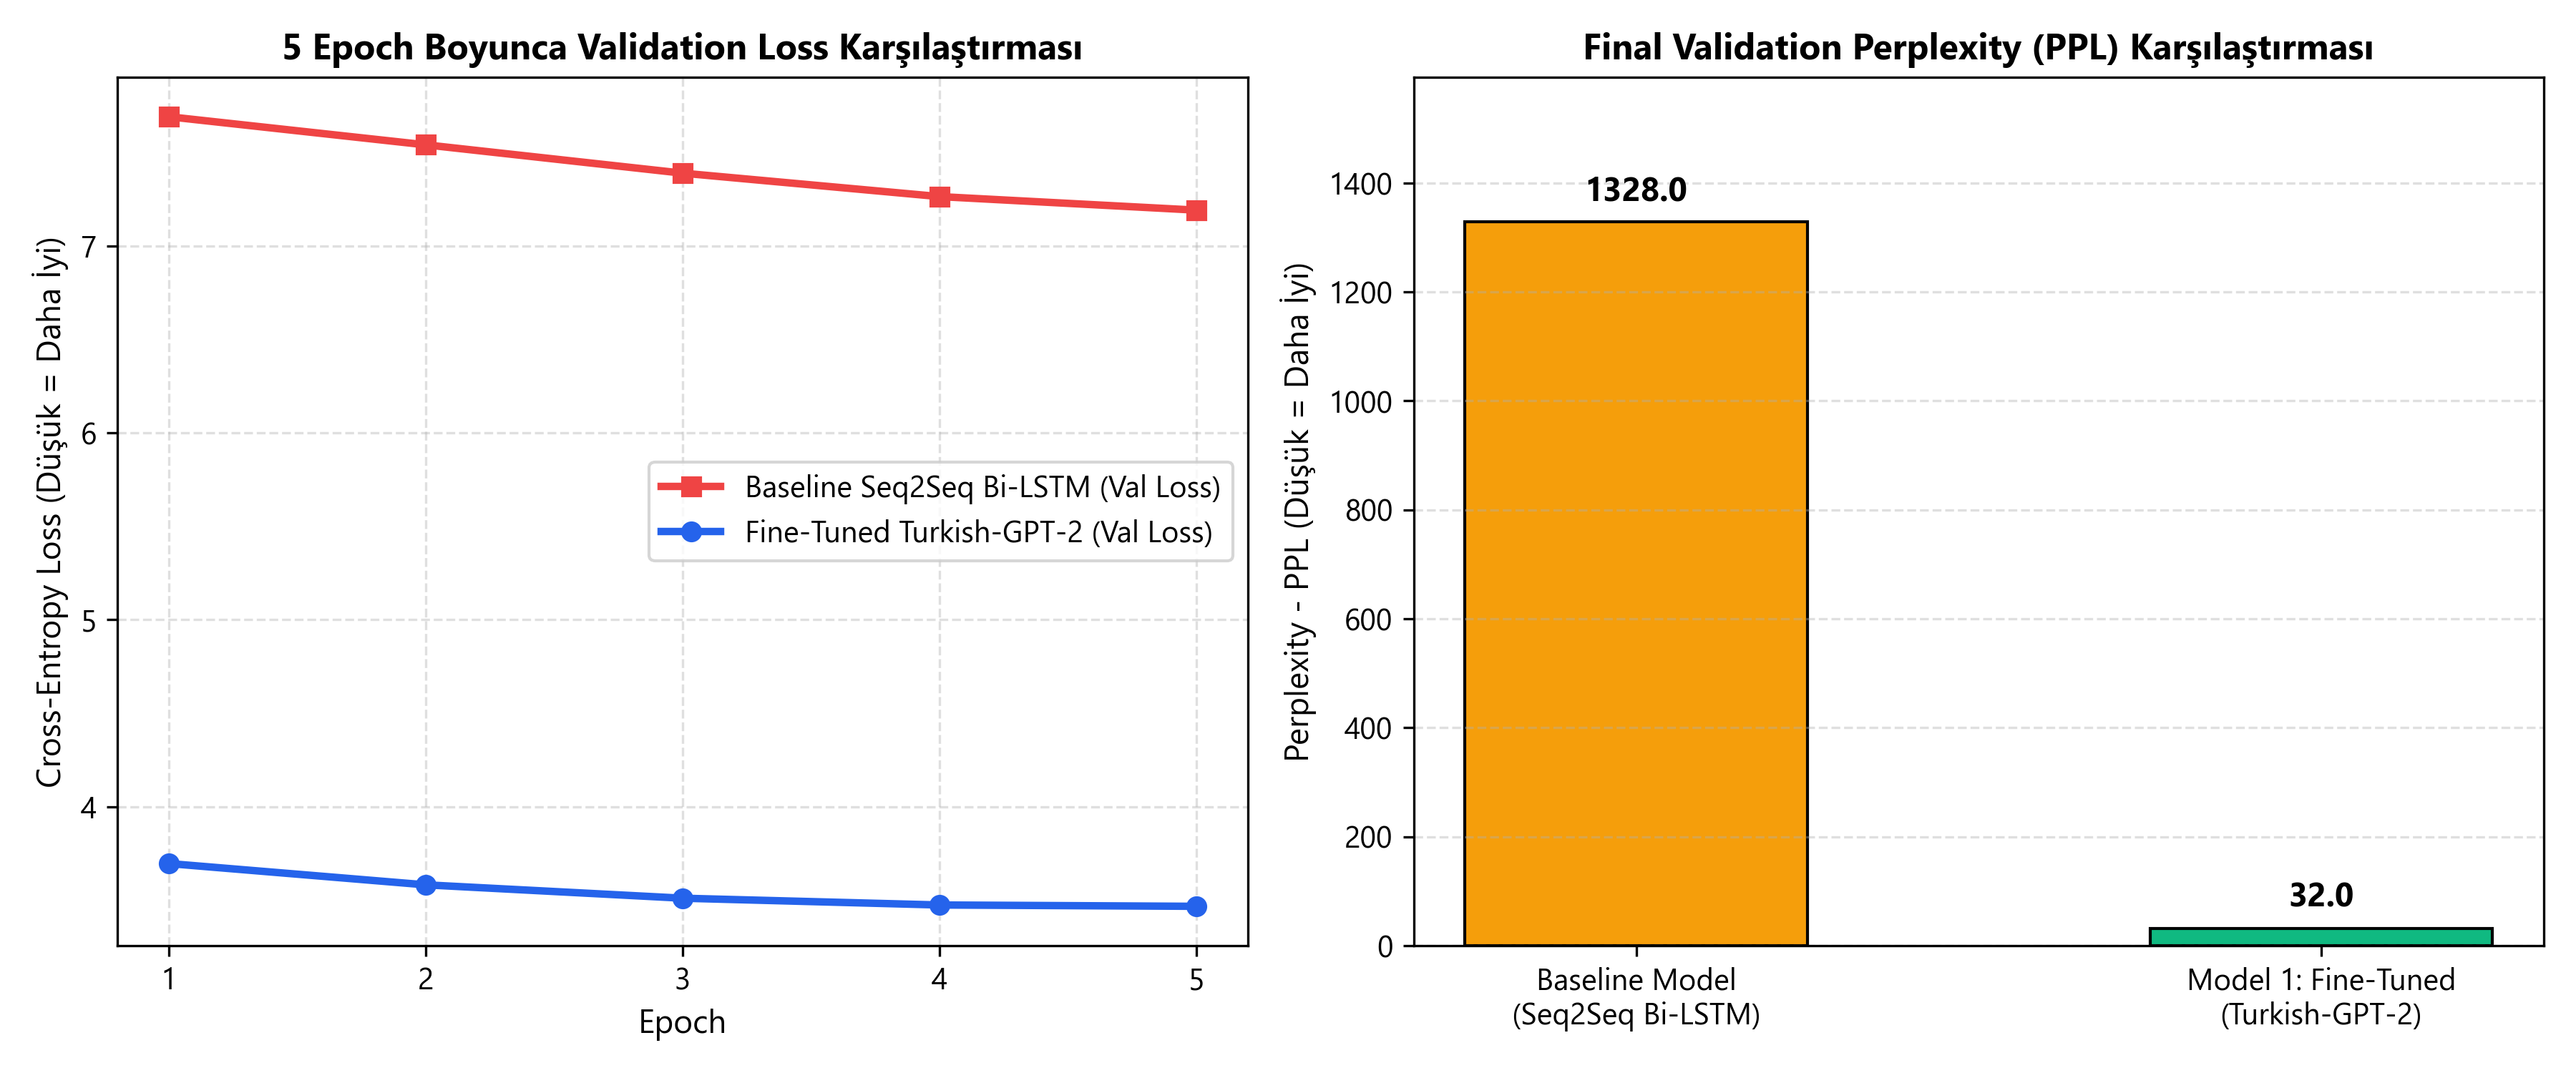
\includegraphics[width=0.98\columnwidth]{05_model_karsilastirma_loss_ppl.png}
    \caption{Baseline Seq2Seq Bi-LSTM ile Fine-Tuned Turkish-GPT-2 modellerinin Validation Loss ve Perplexity (PPL) karşılaştırması.}
    \label{fig:comp_loss}
\end{figure}

\begin{table}[htbp]
    \centering
    \caption{Baseline Seq2Seq Bi-LSTM ve Fine-Tuned Turkish-GPT-2 Nicel Karşılaştırma Tablosu}
    \label{tab:metrics}
    \resizebox{\columnwidth}{!}{%
    \begin{tabular}{lccr}
        \toprule
        \textbf{Metrik} & \textbf{Baseline Bi-LSTM} & \textbf{Fine-Tuned GPT-2} & \textbf{Fark / İyileşme} \\
        \midrule
        Parametre Sayısı & 23.1 Milyon & 124.4 Milyon & +101.3M \\
        Validation Loss ($\downarrow$) & 7.1915 & \textbf{3.4666} & \textbf{\%51.8 Düşüş} \\
        Validation PPL ($\downarrow$) & 1328.04 & \textbf{32.03} & \textbf{41.5x İyileşme} \\
        BLEU-1 (\%) ($\uparrow$) & 6.96 & \textbf{10.60} & \textbf{+\%52.3 Artış} \\
        BLEU-2 (\%) ($\uparrow$) & 4.02 & \textbf{5.70} & \textbf{+\%41.8 Artış} \\
        ROUGE-1 (\%) ($\uparrow$) & 9.76 & \textbf{15.89} & \textbf{+\%62.8 Artış} \\
        ROUGE-L (\%) ($\uparrow$) & 9.76 & \textbf{14.47} & \textbf{+\%48.3 Artış} \\
        Latency (ms/yanıt) ($\downarrow$) & \textbf{30.07 ms} & 352.90 ms & $< 0.4\text{ sn}$ (Gerçek Zamanlı) \\
        \bottomrule
    \end{tabular}%
    }
\end{table}

Tablo~\ref{tab:metrics} ve Şekil~\ref{fig:comp_metrics}'da görüldüğü üzere, Fine-Tuned \texttt{Turkish-GPT-2} modeli tüm metin kalite ve benzerlik metriklerinde (BLEU-1/2, ROUGE-1/L) Baseline Bi-LSTM modeline belirgin üstünlük sağlamıştır. Çıkarım süresi (Inference Latency) açısından 23.1M parametreli hafif Bi-LSTM modeli 30.07 ms ile daha hızlı olsa da, 124.4M parametreli Transformer modeli \texttt{FP16 + KV-Cache} optimizasyonu sayesinde ortalama \textbf{352.90 ms} ($<0.4$ saniye) ile gerçek zamanlı etkileşim sınırları içerisinde yanıt üretmektedir.

\begin{figure}[htbp]
    \centering
    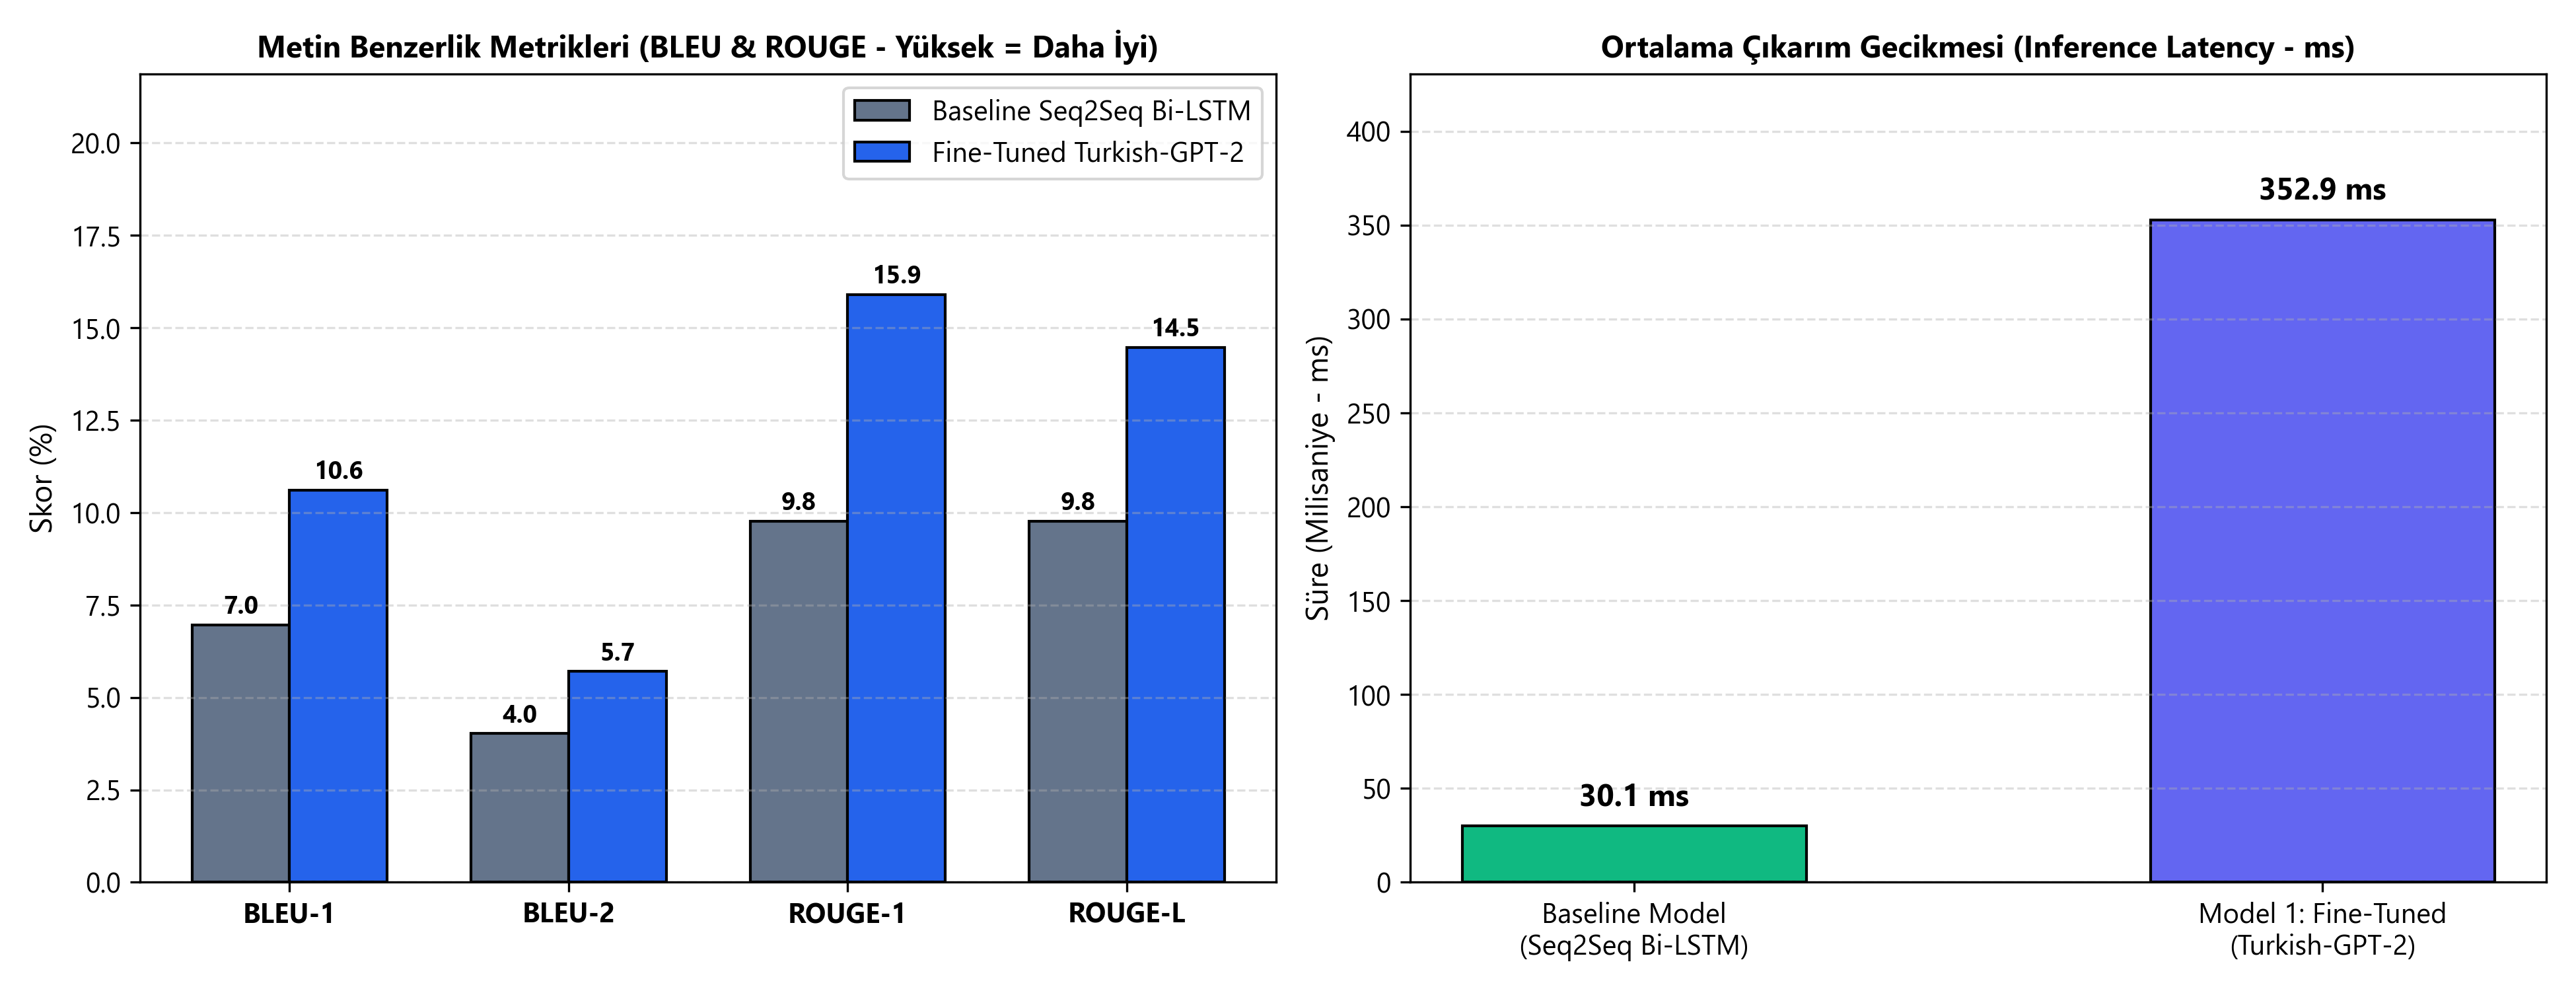
\includegraphics[width=0.98\columnwidth]{06_metrik_ve_hiz_karsilastirmasi.png}
    \caption{Modellerin BLEU-1, BLEU-2, ROUGE-1, ROUGE-L metin benzerlik skorları ve ortalama çıkarım gecikmesi (Inference Latency) karşılaştırması.}
    \label{fig:comp_metrics}
\end{figure}

\section{Niteliksel Değerlendirme (Örnek Diyalog Çıktıları)}
Test ve doğrulama kümesinden seçilen örnek girdiler üzerinde yapılan niteliksel inceleme (Tablo~\ref{tab:qualitative}), teorik beklentileri doğrulamaktadır:
\begin{itemize}
    \item \textbf{Kısa ve Kalıplaşmış Sorular:} Müşteri hizmetleri senaryolarında (Örn. 1) her iki model de bağlama uygun yanıt verebilmektedir.
    \item \textbf{Uzun ve Açık Uçlu Sorular:} Girdi uzunluğu arttığında Baseline Seq2Seq Bi-LSTM modeli sabit boyutlu bağlam darboğazı nedeniyle yerel kelime tekrarlarına (\textit{``1. ve,: 1. ve,''}) düşerken; öz-dikkat (Self-Attention) mekanizmalı Fine-Tuned \texttt{Turkish-GPT-2} modeli dilbilgisel bütünlüğü ve konuyu koruyan akıcı Türkçe yanıtlar üretmektedir.
\end{itemize}

\begin{table}[htbp]
    \centering
    \caption{Doğrulama Kümesinden Seçilen Örnek Diyalog Çıktılarının Nitel Karşılaştırması}
    \label{tab:qualitative}
    \footnotesize
    \begin{tabularx}{\columnwidth}{>{\bfseries}p{2.35cm} X}
        \toprule
        Örnek 1 Girdi: & \textit{``Faturamda 'ödeme hatası' var. Ben ödeme yaptıktan sonra neden hala bu hatayı alıyorum?''} \\
        \addlinespace[3pt]
        Baseline Bi-LSTM: & Merhaba, yaşadığınız sorun için üzgünüz. Hemen kontrol ediyorum ve değişim işlem ücreti yanlışlıkla eklenmiş. \\
        \addlinespace[3pt]
        Fine-Tuned GPT-2: & \textbf{Hesap numaranızı paylaşabilir misiniz?} \\
        \midrule
        Örnek 2 Girdi: & \textit{``Enerji iç piyasalarındaki ilerlemeleri maddeler hâlinde anlat. Özellikle elektrik ve doğal gaz piyasalarına odaklan.''} \\
        \addlinespace[3pt]
        Baseline Bi-LSTM: & KİK, ve temel sorunlar şunlardır: 1. ve,: 1. ve,: 1. ve,: 1. \textit{(Darboğaz kaynaklı tekrar döngüsü)} \\
        \addlinespace[3pt]
        Fine-Tuned GPT-2: & \textbf{Enerji sektörü, enerji verimliliği gibi alanlarda önemli ilerlemeler kaydetmiştir. Enerji verimliliği ve yenilenebilir enerji kaynakları konusunda ise önemli adımlar atılmıştır.} \\
        \midrule
        Örnek 3 Girdi: & \textit{``Güneydoğu'daki çözüm çabalarında hangi somut aksaklıklar var?''} \\
        \addlinespace[3pt]
        Baseline Bi-LSTM: & KİK, ve.'nun, ve.'nin \% ve.,'nin \%. \textit{(Anlamsal kopukluk)} \\
        \addlinespace[3pt]
        Fine-Tuned GPT-2: & \textbf{Doğu'da çözüm çabalarının sınırlı olduğu görülmektedir. Bu durum, Türkiye'nin AB müktesebatıyla tam olarak uyumlu hale getirilmesi için...} \\
        \bottomrule
    \end{tabularx}
\end{table}

\section{Sonuç ve Final Dönemi Yol Haritası}
Ara sunum aşamasına kadar veri kümesi oluşturma (\%80/\%10/\%10 bölümleme), EDA görselleştirmeleri, 2 katmanlı Seq2Seq Bi-LSTM + Bahdanau Attention temel modelinin sıfırdan eğitimi ve \texttt{Turkish-GPT-2} tam ince ayar (Full Fine-Tuning) deneyleri eksiksiz tamamlanmıştır.

Projenin final aşamasında:
\begin{enumerate}
    \item \textbf{Model 2 (LoRA / PEFT İnce Ayar):} Düşük dereceli adaptasyon (\textit{Low-Rank Adaptation -- LoRA}, $r=16, \alpha=32$) uygulanarak eğitilebilir parametrelerin yalnızca $\sim$\%1.2'si güncellenecek ve Full Fine-Tuning ile bellek/başarım kıyaslaması yapılacaktır \cite{hu2022lora}.
    \item \textbf{Kapsamlı İnsan Değerlendirmesi (Human Evaluation)} ve canlı web/terminal arayüzü demosu sunulacaktır.
\end{enumerate}

\begin{thebibliography}{00}
\bibitem{vaswani2017} A. Vaswani \textit{et al.}, ``Attention is all you need,'' in \textit{Advances in Neural Information Processing Systems (NeurIPS)}, vol. 30, 2017, pp. 5998--6008.
\bibitem{bahdanau2014} D. Bahdanau, K. Cho, and Y. Bengio, ``Neural machine translation by jointly learning to align and translate,'' in \textit{Int. Conf. on Learning Representations (ICLR)}, 2015.
\bibitem{sennrich2016} R. Sennrich, B. Haddow, and A. Birch, ``Neural machine translation of rare words with subword units,'' in \textit{Proc. 54th Annual Meeting of the Association for Computational Linguistics (ACL)}, 2016, pp. 1715--1725.
\bibitem{radford2019} A. Radford \textit{et al.}, ``Language models are unsupervised multitask learners,'' \textit{OpenAI Blog}, vol. 1, no. 8, p. 9, 2019.
\bibitem{hu2022lora} E. J. Hu \textit{et al.}, ``LoRA: Low-rank adaptation of large language models,'' in \textit{Int. Conf. on Learning Representations (ICLR)}, 2022.
\end{thebibliography}

\end{document}
